%%%%%%%%%%%%%%%%%%%%%%% file template.tex %%%%%%%%%%%%%%%%%%%%%%%%%
%
% This is a general template file for the LaTeX package SVJour3
% for Springer journals.          Springer Heidelberg 2006/03/15
% Copy it to a new file with a new name and use it as the basis
% for your article. Delete % signs as needed.
% This template includes a few options for different layouts and
% content for various journals. Please consult a previous issue of
% your journal as needed.
%%%%%%%%%%%%%%%%%%%%%%%%%%%%%%%%%%%%%%%%%%%%%%%%%%%%%%%%%%%%%%%%%%%
%
% First comes an example EPS file -- just ignore it and
% proceed on the \documentclass line
% your LaTeX will extract the file if required
%\begin{filecontents*}{example.eps}
%!PS-Adobe-3.0 EPSF-3.0
%%BoundingBox: 19 19 221 221
%%CreationDate: Mon Sep 29 1997
%%Creator: programmed by hand (JK)
%%EndComments
%gsave
%newpath
%  20 20 moveto
%  20 220 lineto
%  220 220 lineto
%  220 20 lineto
%closepath
%2 setlinewidth
%gsave
%  .4 setgray fill
%grestore
%stroke
%grestore
%\end{filecontents*}
%
%\documentclass{svjour3}                    % onecolumn (standard format)
%\documentclass[smallextended]{svjour3}     % onecolumn (second format)
\documentclass[twocolumn]{svjour3}          % twocolumn
%\smartqed  % flush right qed marks, e.g. at end of proof
\usepackage{graphicx}
\usepackage{mathptmx} % use Times fonts if available on your TeX system
% insert here the call for the packages your document requires
\usepackage{latexsym}
% etc.
% please place your own definitions here and don't use \def but
% \newcommand{}{}
% Insert the name of "your journal" with
\journalname{Innovations in Systems and Software Engineering}
%%%%%%%%%%%%%%%%%%%%%%%%%%%%%%%%%%%%%%%%%%%%%%%%%%%%%%%%%%%%%
\begin{document}

\title{From Use-Cases to Test-Cases via Meta-Model-based Reasoning.\thanks{This 
     project is supported by Formal Methods Europe as well as the Research and 
     Development Programme of the University of Pretoria.}}
\subtitle{Position Paper --- Work in Progress}

\titlerunning{From Use-Cases to Test-Cases} % if too long for running head
\author{Stefan Gruner}
\authorrunning{Gruner} % if too long for running head

\institute{S. Gruner \at
              Dept. Computer Science \\
              Universiteit van Pretoria \\
              Republic of South Africa \\
              \email{sg@cs.up.ac.za}}

\date{Received: \today / Accepted: date}
% The correct dates will be entered by the editor

\maketitle

\begin{abstract}
In \emph{Use Cases Considered Harmful}, Simons has analyzed 
the logical weaknesses of the UML Use Case notation and has 
recommended to ``fix the faulty notion of dependency'' \cite{Simons}. 
The project sketched in this position paper is inspired by 
Simons' critique. The main contribution of this paper is a 
detailed meta model of possible relations between Use Cases. 
Later in the project this meta model is then to be formalized 
in a natural deduction calculus which shall be implemented in 
{\sc Prolog}. As a result of such formalization a Use Case 
specification can be queried for inconsistencies as well as 
for test cases which must be observable after a software system 
is implemented based on such a Use Case specification. Software 
tool support for this method is also under development.
\keywords{Use Cases \and Test Cases \and Meta Model \and {\sc Prolog}}
%%%%%%%%%%%%%%%%%%%%%%%%%% \PACS{PACS code1 \and PACS code2 \and more}
%%%%%%%%%%%%%%%%%%%%%%%% \subclass{MSC code1 \and MSC code2 \and more}
\end{abstract}

\section{Motivation and Overview}
\label{sec:intro}
The UML is notorious not only for its commercial popularity but also 
for its vagueness and ambiguity. For this reason various sub-langues 
of the UML have already been subject to the application of precision
enhancing techniques: for example there is the well known OCL in support 
of UML's structural notations (class- and object diagrams), whereas 
a considerable number of papers deals with formal representations 
of UML's state transition diagrams in more precise notations such 
as {\bf B} \cite{butler}.

Rather few papers however (see section `Related Work' below) 
deal with the precision of UML's Use-Case ({\bf UC}) diagrams, 
in spite of popular voices announcing UC diagrams as \emph{the} 
premier language of the UML, upon which everything else depends 
\cite{KGu04}. If UC modeling is really as relevant as it is often 
announced to be, then great care must be taken about the precise 
meaning of a UC specification before any misunderstandings can 
procreate themselves as errors and defects in the software code 
being derived from it. For example, what would it mean for the 
processes of a `live' subject system if an actor could trigger 
a UC which is designed as a mandatory inclusion of another UC? 
Figure \ref{fig:INTRO} depicts such a questionable scenario, 
simply for the sake of stimulating the reader's problem 
awareness.

%\begin{figure*}
% Use the relevant command to insert your figure file.
% For example, with the graphicx package use
%  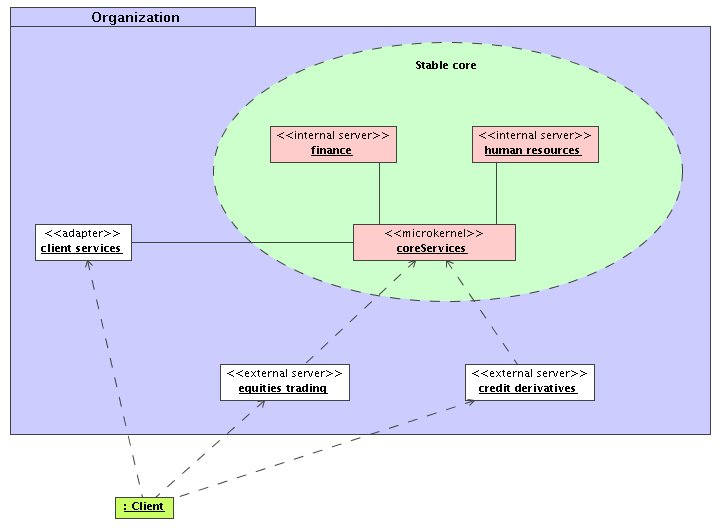
\includegraphics[width=0.75\textwidth]{example.eps}
% figure caption is below the figure
%\caption{Please write your figure caption here}
%\label{fig:2}       % Give a unique label
% \end{figure*}
\begin{figure}[t!]
\begin{center}
\includegraphics[width=8cm]{Fig00}\\   
\caption{\it Motivation: what is the precise meaning of this UC diagram?}
\label{fig:INTRO} 
\end{center} 
\end{figure}

In this context it is interesting to note how the authors of \cite{KGu04}, 
arguing explicitly from a commercial position, \emph{praise} exactly that 
kind of above-mentioned ambiguity and vagueness which the scientifically 
minded software engineer is determined to stamp out. Therefore we\footnote{I 
	am supported by project students: see acknowledgments below.} will not 
take \cite{KGu04} too serious as far as their affinity to vagueness and 
ambiguity is concerned, but we take them serious as far as their emphasis 
of the UML-UC notation as the starting point of user-centred requirements 
engineering in the early phases of a development project is concerned. 

In contrast to the authors of \cite{SACJ35}, who only make a small 
sub set of the UC notation accessible to FDR model checking, we aim 
at a theory for the full UC notation that allows not only for checking 
the internal logical consistency of a UC specification, but shall also 
enables us to ---eventually--- generate high-level Test-Cases directly 
from a consistent UC specification. 

The main contribution of this paper is a rich meta model of possible
relations which could be established between UC or, more precisely,
their process instances. This set of possible relation types exceeds
by far the few relation types which are defined upon UC by the UML.
As soon as this meta model of relations is established, meta relations
(i.e. axioms and rules) can be formulated which enable the search for 
\emph{inconsistencies within} a given UC specification as well as the
search for \emph{implementation consequences} arising \emph{from} the
given specification; these consequences should then be empirically
testable after the system is implemented.

The definition and formalisation of all those consistency rules, 
however, is ongoing project work and, therefore, not in the scope 
of this concept proposal paper any more.
 
\subsection{Method}

We distinguish various UC relations about which we want to reason. 
These relations are classified into the following categories:
\begin{description}
\item[\it Diagrammatic relations] 
 are those ones which are depiced by various types of lines between 
 UC and Actors in the standard UML diagrams \cite{KGu04}. We can 
 also call these relations \emph{explicit} because of their `visual' 
 appearance in the UC diagrams.
\item[\it Modal relations] 
 are those ones (between UC and/or actors) which are newly introduced 
 in our approach, for the sake of enriching the information which is
 transported by a UC diagram between the stakeholders of a software
 development project. In our theory we introduce basdically two new
 modal categories of UC relations, which are:
 \begin{itemize} 
 \item \emph{Temporal}: to reason about `before', `during', and `after'
        in several variations, and 
 \item \emph{Causal}: to reason about `enable', `trigger', 
        pre\-con\-di\-ti\-ons, etc.,\footnote{The standard UML `trigger' 
        relationship between an Actor and a UC, or between two UC, is in 
        fact a causal relationship; however in our model the possibility 
        of building causal expressions is considerably expanded beyond
        this one, simple form of causality.} 
 \end{itemize}
whereby it should be noted that a particular temporal order does not 
necessarily imply a causal one. We also call these relations implicit, 
because they cannot be `seen' in the classical UML UC 
depictions.\footnote{Future work could also be dedicated to hierarchical 
  compositions of UC, which are also not precisely defined in the standard 
  UML, that describe how an `outer' UC can be composed of `inner' UC that 
  are not visible from the outer perspective. This feature, which could be
  graphically depicted by smaller UC `bubbles' being completely contained 
  within a bigger surrounding UC `bubble', similar to inner classes in OOP, 
  would be in support of hierarchic system modeling strategies which make 
  use of abstraction and composition.}
\end{description}
Note that, in principle, a UC could also be somehow related to itself 
in structural recursion, though this is rarely seen in industrial UC 
specifications. Such self-references on the UC specification level 
would have to be adequately interpreted in terms of their actual 
instances during the lifetime of the subject system. For example, 
a UC which $<<$includes$>>$ itself could model a recursive system 
in which a parent process generates child processes of its own kind. 
Or for example, if there is mutual exclusion relation of a UC from 
itself on the level of specification (UC diagram), then we would have 
actually modelled a `singleton pattern' to such an extent that no two 
process instances of that UC can be alive in the subject system at the 
same moment in time.

Consequently we must distinguish clearly between UC as descriptions 
and their process \emph{instances}, in analogy to the distinction 
between classes and their object instances in OOP. For the sake of 
well-behaved software systems derived from such UC descriptions we 
stipulate:
\begin{itemize}
\item
The possible infinity of a system stems from the infinite number of UC 
instances living sequentially or simultaneously over the time, whereas 
each \emph{individual} UC instance is \emph{finite} and must terminate 
after a non-infinite amount of time.
\item
The generation of new UC instances by already existing UC instances, 
which might possibly result in an infinite system, may be of recursive 
nature and are depicted in the UC diagram (at description level) by a 
looping trigger-line from a UC symbol to itself.\footnote{In other words: 
  any sloppy speaking of `an infinite UC' (or something like this) means 
  that terminating instances of such UC can be created again and again, 
  and a `looping' UC would be one in which some instance $u_{i}$ would 
  give birth to a successor instance $u_{(i+1)}$ before terminating 
  itself.}
\item
To each actor role symbol (`stick-man') we assume exactly one singleton 
instance at any time.
\end{itemize}
In the logic description of such an enhanced UC meta model, which 
is needed for consistency checks and property deduction on UC 
specifications, the basic properties will be described by \emph{terms} 
whereas the (meta) relations will be expressed by \emph{predicates}; 
(see below for more explanations).

To be able to relate those categories to UC and actors, we must 
define a meta model that classifies the properties (attributes) 
of them, such as `begin', `end', or other intrinsic states of 
them. In the meta model we regards actors as special cases of 
UC for the sake of theoretical uniformity. Thereby we regard 
the various relationships between UC as extrinsic properties, 
not as their intrinsic states.

The main part of our work will be the establishment of meta 
relations as consistency axioms and rules about the primary 
UC relations. Our approach is `2-dimen\-sional' in the sense 
that it establishes laws (or meta relations) for (at most) 
pairs of relations; in other words: conclusions are drawn
from maximally two premises on top of the conclusion line.
Formally this is the usual rule structure in `natural' 
deduction calculi, and \emph{materially} (w.r.t. a UC diagram) 
this corresponds to a \emph{locality principle} in which only 
small sub graphs of a UC specification graph are under scrutiny 
at the same time.\footnote{Future work, 
  if necessary, may attempt at generalizing our approach 
  from 2-dimensional to 3-dimensional, or even n-dimensional, 
  meta relations respectively consistency rules, which would
  materially correspond to the scanning of larger areas of a
  UC specification graph for patterns of inconsistency.} 
Thus, we will be dealing with set of consistency axioms 
and rules of the following forms (schemes):
\begin{center}
$\frac{UC~\mathcal{R}~UC}{{\it consequence}}$ ~or
~$\frac{\stackrel{UC~\mathcal{R}~UC}{UC~\mathcal{R}~UC}}{{\it consequence}}$
\end{center}
whereby $\mathcal{R}$ are various possible relations in which 
two UC (or, more precisely, their runtime instances) can be found, 
and the {\it consequence} is another description of UC relationships 
or properties that must hold for the sake of the consistency of the 
specification. This will make automated reasoning about an entire UC 
specification possible. Those abstract rule schemes can then be made 
concrete by instantiation, yielding rules which can be implemented 
in {\sc Prolog} in a straightforward manner. 

For Example if we know that $u'$ is a sub UC of $u$ (via the inheritance 
relation $\Longrightarrow$) and $u$ has any property $R$ ---which could 
even be a relation to yet another UC $u''$--- then the automated reasoning 
engine must be able to conclude that $u'$ is in possession of property $R$, 
too, formalized as:
\begin{center}
 $\frac{\stackrel{u' \Longrightarrow u}{u~R~u''}}{u'~R~u''}$
\end{center}
Another example of a consistency rule of this scheme: If an event $e$ 
is happening before another event $e'$, and $e'$ happens before $e''$, 
then $e$ also happens before $e''$.\footnote{For the purpose of this 
	paper we assume to be located in a small region of a Newtonian universe 
	and do not take any Einsteinian considerations of relative time-lines, 
	light-cones, etc., into account.}  

Finally we had to make a decision about how to represent the `ontology' 
of our model: Though we could have chosen some notation developed in the 
field of \emph{Description Logics} (DL) which have attracted considerable 
attention in the `ontology' community, we have chosen to express our model 
directly in the well known executable logic specification language {\sc 
Prolog}, not at least because of nowadays available {\sc Prolog/Java} 
interfaces, which should allow for a comparatively easy integration of 
the executable {\sc Prolog} UC model into a mostly {\sc Java}-implemented 
prototype for the demonstration of the feasibility of our ideas.

\subsection{Use-Cases and their Instances}
Commercial literature on UC modeling, for example \cite{KGu04}, does 
not clearly distinguish between a UC description (represented by an 
oval `bubble' in a UML UC graph) and its actual runtime instances 
which are, in fact, \emph{processes}. This difference is in analogy 
to the relationship between classes and objects in OOP. In a `live' 
software system, more than one process instances could possibly exist 
to any one UC `bubble', either simultaneously at the same time, or 
sequentially at different points of time, or even in a combination 
of both. Consequently, if ($u~\mathcal{R}~u'$) is a relationship 
defined in a UC specification, we will have to reason especially 
about the consequences of $\mathcal{R}$ as far as the process 
instances of $u$ and $u'$ are concerned. For this reason our 
model will also make use of the usual existential and universal 
quantifiers (on UC instances), as it is further described in the 
remainder of this paper.

%%%%%%%%%%%%%%%%%%%%%%%%%%%%%%%%%%%%%%%%%%%%%%%%%%%%%%%%%%%%%%%%%
\section{Use-Case Meta-Model}
\label{sec:meta}
As the detection and formalisation of valid consistency rules on
UC specifications, as mentioned above, is still ongoing work in 
its early stages, the main contribution of this proposal paper
is the definition of a meta model which shows (and structures)
the `pool' of all possible relations between (or properties of)
UC. These relations can be used to instantiate the materially 
empty rule \emph{schemes} (introduced in the previous section) 
in order to obtain the concrete applicable consistency rules 
on which the operations of the planned UC reasoning engine 
are based.

To reason formally about a UC model, a number of attributes must 
be introduced to a UC in the fashion of an `ontology'. Whilst some 
of those attributes will be \emph{static} in nature (for example, 
some UC could be a mandatory or optional to sub-UC to some other 
UC, which is always the case) other UC properties are of dynamic 
nature in the sense that their value can change during the lifetime 
of a UC instance. For example, temporal reasoning about one UC 
instance happening before or during of after another UC instance
does only make sense if there exist a changeable state attribute 
value which reflects the `ticking of time' during the lifespan of 
a UC instance. In the following, we present our meta model at two 
conceptual levels:
\begin{itemize}
\item
A \emph{class diagram} shows what types of entities (e.g. normal 
UC or Actors) we have and which kinds of attributes they carry:
\begin{itemize}
\item
Whereas some attributes represent \emph{unary} relations (e.g. 
internal values such as instance birth time) other attributes 
represent \emph{binary} relations between two entities.\footnote{UC 
	nesting would be even $n$-ary.}
\item
Whereas some attributes in the meta model represent \emph{standard} 
relations between UC according to the UML (which we also called the 
\emph{diagrammatic} ones), other relational attributes represent 
the new contributions of our meta model; these are also called the 
\emph{modal} ones.
\end{itemize}
\item
Then, on a conceptually finer level, possible values of the \emph{dynamic} 
(time related) attributes are defined in terms of a simple \emph{finite 
state machine}.
\begin{itemize}
\item
The different states of a UC evolving over time allow for finer temporal 
modelling; e.g. we cannot only say: `this UC happens before that UC' but 
we could also say more precisely, for example: `this UC terminates after 
that UC has started', or something like this. 
\end{itemize}
\end{itemize}
As mentioned above, all UC instances are regarded as `mortal' and finite 
in time, and the possibly infinity of a subject system would result from 
the unlimited creation of such finite instances --- `unlimited' either 
in the number of instances simultaneously existing at any particular 
point of time, or unlimited as far as the life span of the entire system 
is concerned (possibly with only a finite number of instances existing 
at any point in time); this is probably the practically relevant case. 

Anyway, this reduction of infinity to finite instance components allows us 
to model any UC instance as a simple state machine as shown below. Thereby, 
the internal states of such a UC machine are the above-mentioned basic (unary) 
properties that underly the modal reasoning about the various relationships of 
UC amongst each other. Moreover, our notion of a `successfully terminated' UC 
instance ---in contrast to an `aborted' one--- may include the generation of 
\emph{data} which might be used as input by other UC instances. According to
the learned practice of software engineering, our model deliberately abstracts 
away from such detail at this early stage of requirements engineering.

As far as the Actors are concerned, we follow the usual UML convention 
accordig to which the Actors represent the \emph{external world}, from 
the system's perspective. Therefore we do not assume anything about 
Actors except their unlimited existence and ability to act; consequently 
we do not attribute any internal states to them.

\subsection{Top Layer of the Meta Model}
\begin{figure}[t!]
\begin{center}
\includegraphics[width=8cm]{Fig01}\\   
\caption{\it Meta Model: Use Cases, Actors, Relations, and States}
\label{fig:1} 
\end{center} 
\end{figure}
Figure \ref{fig:1} shows the top layer of our UC meta model. 
The central concept is, indeed, the relation, and not the UC 
itself. The picture of Figure \ref{fig:1} is explained as 
follows:
\begin{description}
\item[\it Relations] have entities, which they `bind' together, 
as well as ---possibly--- some quantification (existential 
or universal) as far as the instance processes to the participating 
entities are concerned. Sub-classes of relations will be shown and 
explained later in this paper; ditto for the possible sub-classes 
of instance-quantification where applicable.
\item[\it Entities] have time attributes representing their `birth'
and `death' of UC instances. These time attributes allow for 
reasoning about `before' or `after' relationships, etc.
\item[\it Actors] are entities which are represented by the well known 
`stick-men' in the pictorial UC diagrams. Belonging to the \emph{external
world} outside the system boundaries, we cannot attribute any system 
properties to them. They are assumed to be always available, thus 
for any actor instance we assume Actor.\emph{birth} $= -\infty$, 
and Actor.\emph{death} $= +\infty$.
\item[\it Use-Cases] are the system-internal entities which are 
represented by the well-known `bubbles' in a UC specification. The 
lifetimes of their process instances are limited, thus we have $0 
\leq$ (p.\emph{death} - p.\emph{birth}) $< \infty$ for every UC 
instance p. Moreover, every UC instance can go through a sequence 
of states during its lifetime (as further explained below); therefore 
a process state class is associated with the UC class in our meta 
model.\footnote{Not depicted in the UC concept of Figure \ref{fig:1} 
	are the other internal UC attributes which are usually found in 
	a UC specification, such as: pre-condition, post-condition, etc. 
	\cite{KGu04} --- some of them are modeled explicitly as relationships, 
	as shown in the following sections below.}
\end{description}

\subsection{Inner Structure of Use-Cases}

A UC is more than a `bubble' in a UC diagram; it has an inner 
structure which, according to the industrial literature \cite{KGu04}, 
comprises the following attributes: Name, Model Iteration Phase, 
Summary, Basic Course of Events, Alternative Paths, Exception Paths, 
Extension Points, Triggers, Assumptions, Pre-Conditions, Post-Conditions, 
Related Business Rules, Author, and Date. 

In non-rigorous forms of UC modeling, the values of these UC attributes 
are simply text strings (though some algorithmic aspects of a UC can also 
be expressed in terms of state machine notations which are offered by other 
formalisms of the UML notation). Moreover, the conceptual difference between 
`Assumptions' and `Pre-Conditions' in \cite{KGu04} is typically vague, 
as is the conceptual difference between `Pre-Conditions' and `Triggers' 
in the informal approach to UC modelling. 

In our model, only the following few of those UC attributes are explicitly 
represented for the purpose of consistency checking and logic reasonning at 
a high level of conceptual abstraction:
\begin{itemize}
\item Any UC's \emph{Basic Course of Events} is abstractly represented 
      by a simple finite state machine (as further described below).
\item \emph{Triggers} and \emph{Pre-Conditions} are represented by 
      external UC relationships which belong to some sub-classes of 
      the Relation class of Figure \ref{fig:1} (as further described 
      below).
\end{itemize}
Post-Conditions are \emph{not} explicitly modelled here for two reasons: 
(i) in most cases, the post-condition of one UC will be the pre-condition 
of another UC, and (ii) in many cases the post-conditions make statements 
about the data configuration of the to-be-modelled subject system; however 
we do not take subject (system) data into account at all at this high level 
of meta modelling. 

\begin{figure}[t!]
\begin{center}
\includegraphics[width=8cm]{Fig02}\\   
\caption{\it Finite State Machine Model of a UC Instance: These States
             are Attributes of the UC Class in the Meta Model}
\label{fig:2} 
\end{center} 
\end{figure}
Figure \ref{fig:2} depicts the abstract state transition diagram to every 
UC instance (process) of a `living' subject system. For the sake of reasoning 
about a UC spacification, the meta model automaton also contains a virtual 
`ghost' state \emph{before} the actual `birth' of a UC instance in the subject 
system. Thus, in our theory, a UC instance is regarded as `virtually' existent 
as soon as it is enabled (i.e. its Pre-Condition is fulfilled), whereas it 
is actually existent only after being triggered by an actor (from outside 
the system boundaries) or by a parent process (from within the subject system). 
Successful termination will eventually occur,\footnote{This could include the 
	production of data, which is however not explicitly modeled by our high-level 
	model. Moreover, we would assume the fulfillment of any post-conditions, which 
	our theory does not model explicitly either, only in this successful termination 
	state.} 
unless the process is halted either by internal failure or by external abortion 
(triggered by an actor from outside the system boundaries). As explained above, 
no UC instance can thus `live' forever, though the subject system as a whole 
could well `live' forever by giving birth to process instances in arbitrary 
numbers. Of course, transition $s$ from $E$ to $R$ in Figure \ref{fig:2} 
could also be induced by another UC via an $<<$include$>>$ or $<<$extend$>>$ 
relationship --- this should be obvious to any reader with some experience 
in UC modelling and does not need any further mentioning.

\subsection{Classical Instance-Quantified Relation Types}

In our meta model, all relationships between UC `bubbles' 
in a UC specification are \emph{binary} and \emph{directed}. 
As a UC `bubble' is only a representation of its extension
(set of instances) the question arises how a relation 
$u~R~u'$ between to UC $u$ and $u'$ should be interpreted
in their extensions $e(u)$ and $e(u')$. This needs to be
further specified by the designers of the subject system.

For this purpose, every relation $R$ in the meta model is 
attributed with two quantifiers: one for the domain side 
of the relation, and one for the range side of the relation, 
thus:
\begin{center} 
$R^{Q}_{Q'}$ 
\end{center}
whereby $Q, Q' \in \mathcal{Q}$ $= \{\forall, \exists, 
\exists!, \not\exists\}$. In other words, $\mathcal{Q}$ 
is the set of the four classical syllogistic quantifiers
`one' ($\exists!$), `some' ($\exists$), `none' ($\not\exists$), 
and `all' ($\forall$).

Example: Given two UC $u$ and $u'$, their extensions 
$e(u)$ and $e(u')$ and a UC relation $R$ relating $u$ 
and $u'$ to $u~R~u'$, then the process instance relation
\begin{center} 
$e(u)~R^{\exists!}_{\forall}~e(u')$\\
would be interpreted as:\\
$\exists! p\in e(u): (\forall p'\in e(u'): p~R~p')$,
\end{center}
whereby $p$ and $p'$ are runtime instances (processes) of UC within 
a `living' subject system. The reader can easily imagine that many 
useful \emph{relation types} can be stipulated in this way, including 
injection, bijection, surjection, the complete relation (`all-to-all'), 
etc.

In this context we conjecture that UC specifications can be made 
more precise and testable by quantifying UC relationships in the 
form of above. Figure \ref{fig:3} depicts the corresponding part 
of the meta model: note the self-association of the super-class 
which denotes the binary pairing of those four classical extension
quantifiers.
\begin{figure}[t!]
\begin{center}
\includegraphics[width=8cm]{Fig03}\\   
\caption{\it Part of the Meta Model defining the
         Instance Quantifications of UC Relations}
\label{fig:3} 
\end{center} 
\end{figure}

\subsection{UC Relations defined by the UML}

The relations between UC and/or actors can be further classified 
in the lower layers of our our meta model. There are, of course, 
the canonical relationships which are well known from the standard 
UML literature:
\begin{description}
\item[\it Inheritance], similar to class-inheritance in OOP, 
 either between two actors or between two UC, but never `mixed'.
 A precise UC inheritance semantics has been suggested by Pierre 
 Metz in \cite{Metz-PhD}.
\item[\it Triggering] in which an actor instance invokes a UC instance 
(via state-transition $s$ according to Figure \ref{fig:2} of above). In 
our meta model, this canonical triggering relationship will be divided 
into further cases (as esplained below).
\item[$<<$extend$>>$] with an implicit deontic modality `optional', 
 between UC only.
\item[$<<$include$>>$] with an implicit deontic modality `mandatory', 
 between UC only.
\end{description}
As soon as two entities (UC and/or actors) are `connected' via any of 
these relations, we can start to reason logically about the consistency 
(meta) relations which must hold as far as the other properties of the 
thus connected entities are concerned. In addition to those canonical 
UC relations we also want to reason about the modalities of causality 
and time-order (relative time of entities to each other, not absolute 
time in terms of numeric values), for which we introduce the according 
new sub-classes to the relation class in our meta model, too. 

As far as the canonical \emph{triggering} (of UC by actor) is concerned, 
we introduce a new distinction between \emph{start}-triggering (state 
transition $s$ in Figure \ref{fig:2}) and \emph{abort}-triggering (state 
transition $a$ in Figure \ref{fig:2}) whereby the start-trigger can be 
further qualified in terms of two deontic modalities name\-ly `mandatory' 
(actor \emph{must} invoke an instance of this UC at some point in the 
lifetime of the subject system), or `optional' (actor \emph{may} invoke 
an instance of this UC). The deontic qualification of the abort-trigger, 
on the other hand, would always be `optional', because it does not make 
sense in practice to abort any running UC instance in every case. 

\begin{figure}[t!]
\begin{center}
\includegraphics[width=8cm]{Fig04}\\   
\caption{\it Classification of Temporal and Causal Relations}
\label{fig:4} 
\end{center} 
\end{figure}
Figure \ref{fig:4} shows the corresponding layers of the meta model,
whereby the canonical concepts are depicted in green colour. Note 
that most of the canonical relations are also causal ones, which is 
depicted by the multiple inheritance of meta model concepts in Figure 
\ref{fig:4} (see blue lines).

\subsection{Temporal Relationships}

Distinguishing for each UC instance a start time and a stop time as 
explained in Figure \ref{fig:2} (i.e. no non-terminating instances), 
two UC instances can only be found in any one of the following time
relations which are depicted in Figure \ref{fig:5}. If two UC symbols 
are given in a UC specification diagram, the software engineer should 
be able to stipulate one of these relations upon them such that further 
reasoning about their process instances becomes possible. It is obvious 
that an `After' relation is only the inversion of the `Before' relation 
(i.e. $p~A~p'$ if and only if $p'~B~p$); therefore no `After' relation 
is shown in Figure \ref{fig:5}. In the meta model, all relation types 
($A, \ldots G$) shown in Figure \ref{fig:5} are sub-classes of the 
Temporal class of Figure \ref{fig:4}. 
\begin{figure}[t]
\begin{center}
\includegraphics[width=8cm]{Fig05}\\   
\caption{\it Different Sub-Classes of Temporal Relations}
\label{fig:5} 
\end{center} 
\end{figure}

\subsection{Causal Relationships}

Figure \ref{fig:4} shows a yet un-expanded super class of the meta model 
for Causal relations, which needs further refinement. Thereby the notion 
of causation must relate not only to the entities (UC or Actors) themselves 
(which can receive or trigger causation) but also to the states of the 
process machine model (of the UC instances) as depicted in Figure \ref{fig:2} 
--- in other words: we want to be able to distinguish causations of `Start', 
causations of `Stop', etc. These are in fact \emph{actual} (i.e. physical) 
triggers. Moreover, following \cite{KGu04}, we also know \emph{conditional} 
(i.e. logical) causations, which enable or prevent the actual triggering of
a process without actually doing the triggering. 

Figure \ref{fig:6} concludes our presentation of the new meta model with 
the full expansion of the Causation class. Also remember that there is 
an extensional `overlap' between the causation class and the canonical 
(UML-defined) relation types; for example the UML relationship between 
an actor and a UC is a causal relationship; those are all actual ones, 
not conditional ones.
\begin{figure}[t!]
\begin{center}
\includegraphics[width=8cm]{Fig06}\\   
\caption{\it Different Types of Causal Relations}
\label{fig:6} 
\end{center} 
\end{figure}

\subsection{Deontic Qualities}

Deontic Logics can describe what `may' or `must' or `must not' be done. 
For example an actor $a$ may trigger this UC, but must not trigger that 
UC, which could be relevant as far as access (login) permissions and 
other security features of a software system are concerned. For our
project we had to decide whether or not to explicitly introduce deontic 
classes into our meta model (and associate them to various entities and 
relationships). However, it turned out that those deontic qualities are 
already \emph{implicitly} modeled by the instance quantifications $mathcal{Q}$
described above, such that no further classes need to be added to the meta 
model for this purpose.
For example, if an actor $a$ may or may not (optionally) trigger some UC 
$u$ via a trigger relation $T$ ---thus: $a~T~u$--- then $T$ could get in 
some form existentially quantified (rather than all-quantified) in order 
to express this optionality of the action. 

\subsection{Negation}

Except of the $\not\exists$ quantifier in $\mathcal{Q}$, negation is 
generally expressed implicitly, namely by omission, in our model. For 
example, if there is \emph{no} trigger relation between a particular 
actor $a$ and a particular UC $u$, then we may conclude that $a$ must 
not trigger $u$ under any circumstances. For the {\sc Prolog}-based
reasoning `behind' such a UC specification we would thus work with 
{\sc Prolog}'s well known \emph{negation-by-failure} semantics.

\section{Ongoing Work in this Project}

After having outlined an elaborate meta model of the UC language in 
the previous section, we must now state what we want to do with it
in the next phases of our project

\subsection{Meta Relations}

Meta relations are consistency axioms and consistency rules about the 
relations which are defined in the meta model of the previous section. 
With all those many relations available the combinatorial possibility 
for such consistency rules are large and it will take time and effort 
to discover the relevant and useful ones before they can be formalised
and implemented. The \emph{difficulty} of this rule finding exercise 
stems from two sources:
\begin{itemize}
\item We want to reason about \emph{testable} UC \emph{instances} 
(i.e. processes at runtime) rather than the abstract UC `bubbles' 
which only represent those instances at the highest possible level 
of abstraction.
\item The relationships about the UC instances (processes) are quantified 
 (universally or existentially) on either side of the binary relationship, 
 which multiplies the number of potential rule candidates to be examined 
 for validity.
\end{itemize}
Once a valid consistency rule has been found, its implementation in 
{\sc Prolog} (or any other deduction language for that matter, such 
as {\sc OPS5}) should be a rather straightforward exercise. Once the 
rules are implemented, it shall be possible
\begin{itemize}
\item to \emph{detect} logical flaws within a UC specification 
 \emph{before} any software development takes place, and
\item to \emph{query} the {\sc Prolog} model with regard to properties 
 of UC instances which must hold \emph{after} the software development 
 has taken place. Then we could ask questions such as: ``is it true
 that all instances of UC $u$ must terminate before any instance of 
 UC $u'$ can be born?'' In other words, we shall be able to generate 
 \emph{test cases} directly from a UC specification. 
\end{itemize}

\subsection{Graphical User Interface of a Prototype}

To make the UC specification system more user-friendly for the 
industrial practitioner, its logic engine should be `hidden' behind 
a graphical user interface. The idea is that the user should be able 
to `attach' the additional specifications (as defined by our meta model) 
to a graphical UC specification which consists mainly of the typical 
`stick-men' and `bubble' diagrams. Such an enhanced UC specification 
must then be translated into \emph{textual form} (in an XML-like 
formalism similar to \cite{Bis} \cite{Rout}) such that it becomes 
amenable to (text-based) automated reasoning. 

From the XML representation of a logically enriched UC specification 
we could then derive the facts on which the {\sc Prolog} engine can 
start its work. The technical (not so much scientific) challenges in 
this scenario are thus:
\begin{itemize}
\item	to extract {\sc Prolog} facts from a mainly graphical, logically
 enhanced UC specification,
\item to couple a {\sc Java}-implemented UC-Editor with an underlying 
 {\sc Prolog} interpreter, and
\item to propagate graphical (`visual') information back into the 
 graphical UC specification editor after the {\sc Prolog} reasoning 
 process has discovered any inconsistency in a UC specification; for 
 example to highlight a logically impossible specification element 
 in red colour, or something like this.
\end{itemize}

\subsection{Nested Use-Cases}

Our meta model does not contain an $n$-ary nesting relation on UC which 
would allow for drawing smaller UC `bubbles' \emph{within} a larger `bubble' 
of a \emph{higher-order} UC. Higher-order (or nested) UC are explicitly 
discouraged by \cite{KGu04}, but nevertheless we think that they might 
be useful for the purpose of top-down system modeling at different levels
of abstraction. Future work would have to expand the meta model as well as 
the set of consistency rules into this direction; thereby the logic rules 
for nested UC would probably have the character of \emph{refinement} rules.

\subsection{Related Work and Literature Studies}

Though we have reason to believe that our approach is quite original, 
we are aware that we are not operating in an un-explored void. In our 
yet ongoing literature studies we have found a number of interesting 
papers which are pointing into the direction of which our project is 
going. For example, the application of \emph{Modal} and \emph{Deontic 
Logic} in Computer Science and Software Engineering is studied by 
\cite{Den} \cite{Kola} \cite{Mai} \cite{Seger}. Another \emph{ontology} (meta-model) approach to UC reasoning can be found in \cite{Gen}. 
Approaches to giving \emph{process semantics} to UC specifications 
can be found in \cite{Back} \cite{Kot} \cite{Li}. 

\section{Summary}

%-----------------------------------------------HERE-----------------

This position paper (category: work in progress) outlined 
a project towards making UC specifications ---previously 
considered harmful \cite{Simons}--- more useful and less 
ambiguous. This shall be achieved by a rich arsenal of UC 
relations, which exceeds by far the small set of UC relation 
types defined by the UML. A more or less fully elaborated 
\emph{meta model} of such relations has been provided 
in this paper as its main contribution. As soon as the 
consistency rules (meta relations) on these rules are 
discovered and formalised, logic reasoning about UC 
specification will be possible. The objective of such 
reasoning is twofold, namely to \emph{detect} logical 
flaws within a UC specification itself (\emph{before} 
system implementation), and to \emph{query} a UC 
specification for test cases which must hold empirically 
(\emph{after} system implementation).
\begin{acknowledgements}
I would like to thanks my student helpers \emph{Ezra Jivan} 
and \emph{Pierre-Henri Kuate} for their efforts with the 
implementation of the prototype, as well as for their 
help with the literature search. Ezra Jivan is also 
helping with the discovery of valid consistency rules 
over the domains of UC relations as outlines in the meta 
model. \emph{Formal Methods Europe} (FME) and the 
\emph{University of Pretoria} are supporting this project 
financially. The \emph{P-UML} (precise UML) community has 
provided valuable hints about literature and related work. 
Last but not least thanks to the anonymous reviewers of 
the UML$+$FM'08 Workshop for their critique; it has been 
taken into account for this published version of our paper.
\end{acknowledgements}
%%%%%%%%%%%%%%%%%%%%%%%%%%%%% BibTeX users please use one of
%\bibliographystyle{spbasic}% basic style, author-year citations
%\bibliographystyle{spmpsci}% mathematics and physical sciences
%\bibliographystyle{spphys} % APS-like style for physics
%\bibliography{}            % name your BibTeX data base
% Non-BibTeX users please use %%%%%%%%%%%%%%%%%%%%%%%%%%

\begin{thebibliography}{}

\bibitem{Back}
R.J. Back \& L. Petre \& I.P. Paltor: 
\newblock Formalizing UML Use Cases in the Refinement Calculus. 
\newblock Technical Report TUCS-TR-279, 1999.		

\bibitem{Bis}
V. Bisova \& K. Richta: 
\newblock Transformation of UML Models into XML. 
\newblock ADBIS-DASFAA Symp., pp. 33-45, 2000.

\bibitem{Den}
N. den Haan: 
\newblock Investigations into the Application of Deontic Logic. 
\newblock LNCS 897, 1995.		

\bibitem{Gen}
G. Genilloud \& W.F. Frank:
\newblock Use Case Concepts using a Clear, Consistent, Concise Ontology. 
\newblock Journal of Object Technology 4/6, 
\newblock Special Issue: Use Case Modeling  at UML-2004.

\bibitem{Kola}
G. Kolaczek: 
\newblock Application of Deontic Logic on role-based access control. 
\newblock Journ. Appl. Math. and Comp. Sc., 2002.		

\bibitem{Kot}
Y. Kotb \& T. Katayama: 
\newblock A Novel Technique to verify UML Use Case Diagrams. 
\newblock IASTED Conf. on Softw. Eng., pp. 300-305, 2006.
		
\bibitem{KGu04}
D. Kulak \& E. Guiney: 
\newblock Use Cases --- Requirements in Context. 
\newblock Addison Wesley / Pearson, 2$^{nd}$ ed., 
\newblock 2004.

\bibitem{Li}
L. Li: 
\newblock Translating Use Cases to Sequence Diagrams. 
\newblock Proc. ASE, pp. 293-296, 2000.

\bibitem{Mai}
T. Maibaum \& S. Khosla \& P. Jeremaes: 
\newblock A Modal Action Logic for Requirements Specification. 
\newblock Softw. Eng. 86, 1986.		

\bibitem{Metz-PhD}
P. Metz:
\newblock Revising and Unifying the Use Case Textual and 
          Graphical Worlds.
\newblock PhD Thesis, promoted by W. Weber \& J. O'Brien,
\newblock Department of Computing,
\newblock Cork Institute of Technology, 
\newblock Ireland, 2004.

\bibitem{Rout}
N. Routledge \& L. Bird \& A. Goodchild: 
\newblock UML and XML Schema. 
\newblock Proc 13$^{th}$ Austr. DB Conf., 
\newblock pp. 157-166, 2002.

\bibitem{SACJ35}
K. Ryndina \& P. Kritzinger: 
\newblock Analysis of Structured Use Case Models
 through Model Checking. 
\newblock South-African Computer Journal 35,
\newblock pp. 84-96, 2005.

\bibitem{Seger}
K. Segerberg: 
\newblock A Deontic Logic of Action. 
\newblock Studia Logica 41, 
\newblock pp. 269-282, 1982.		

\bibitem{Simons}
A. Simons: 
\newblock Use-cases considered harmful. 
\newblock 29$^{th}$ Conf. on Techn. of OO Lang. and Syst., 
\newblock pp. 194-203, 1999.

\bibitem{butler}
C. Snook \& M. Butler:
\newblock UML-B and Event-B --- An Integration of Languages and Tools.
\newblock Proc. IASTED Internat. Conf. on Softw. Eng. (SE2008),
\newblock Innsbruck (A), February 2008.

\end{thebibliography}
\end{document}
% end of file template.tex

